\documentclass[11pt,a4paper]{article}
\usepackage[utf8]{inputenc}
\usepackage[T1]{fontenc}
\usepackage{amsfonts}
\usepackage[french]{babel}
\frenchbsetup{StandardLists=true} % à inclure si on utilise \usepackage[francais]{babel}
\usepackage{enumitem}
\usepackage{amssymb}
\usepackage{amsmath}
\usepackage[left=2cm,right=2cm,top=2cm,bottom=2cm]{geometry}
\usepackage{multirow}
\usepackage[dvipsnames]{xcolor}

\usepackage[T1]{fontenc}
\usepackage{fouriernc}
\usepackage{graphicx}

\usepackage{setspace}
\singlespacing

\usepackage{pstricks}
\usepackage{xkeyval}
\usepackage{pst-labo}


\usepackage{multicol}
\usepackage{caption}
\usepackage{fancyhdr}
\pagestyle{fancy}
\renewcommand\headrulewidth{1pt}
\fancyhead[L]{Lycée Denis Diderot }
\fancyhead[R]{Classe de 1 Bac Pro }
\setcounter{page}{1}\fancyfoot[C]{page \thepage}
\fancyfoot[R]{Année 2025-2026}
\fancyfoot[L]{Alexis RUIZ}
\usepackage{multirow,tabularx,booktabs}
\newcommand{\cadreblanc}[1]{%
\medskip\framebox[\linewidth][c]{%
\rule{0mm}{#1mm}}\par
\medskip}

\usepackage{awesomebox}
\setlength{\aweboxvskip}{0mm}
\usepackage{pifont}
\usepackage{chemmacros}
\chemsetup{modules=all}
\setlength{\columnseprule}{.25mm}

\renewcommand{\arraystretch}{2}
\newcommand*\acocher{\quitvmode{\fboxsep0pt \fboxrule0.8pt \fbox{\vrule height1.8ex depth.1ex width0pt \vrule height0pt depth0pt width1.9ex }}}

\newcommand{\code}{\awesomebox[black]{2pt}{

\includegraphics[scale=0.15]{../Chapitre 1 - Energie et puissance électrique/images/frame.png}
}{black}}

\newcommand{\moteur}{\awesomebox[black]{2pt}{

\includegraphics[scale=1]{images/moteur.jpg} 
}{black}}

\newcommand{\defconclusion}{\awesomebox[black]{2pt}{\rotatebox{90}{\Large{\textbf{Conclusion}}}}{black}}

\frenchbsetup{StandardLists=true}



\begin{document}

\flushleft \textbf{NOM :\\
Prénom:\\[0,4cm]
}
\hrule\


\begin{center}
 \LARGE{Activité 1 - Pourquoi la vitesse varie-t-elle durant un saut ?   }
\end{center}



\normalsize

\hrule\
\\[0,2cm]
   \begin{center}
   \textbf{Le soin et la rédaction interviendront dans la notation.}
   \end{center} 

\noindent%
\begin{minipage}{.5\textwidth}%
 
 Pendant la chute libre de Felix Baumgartner, sa vitesse (en m/s) est relevée toutes les 5s, pendant les 260 premières secondes avant qu'il ouvre son parachute. 
 
\end{minipage}%
\hfill
\begin{minipage}{.45\textwidth}%
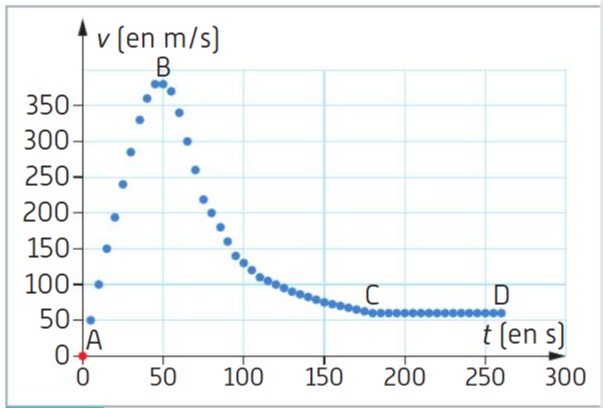
\includegraphics[width=\textwidth]{images/doc1.png}
\end{minipage}%

\vfill

  \ding{202} Lisez sur le graphique entre quels points Félix Baumgartner est en cours d'accélération, de décélération, sans accélération  et sans ralentissement.\\
  \begin{multicols}{3}
  \cadreblanc{40}
  \cadreblanc{40}
  \cadreblanc{40}
  \end{multicols}

  \vfill 

  \ding{203} Expliquez les variations de vitesse durant la chute 
  \cadreblanc{30}
   
\vfill 
  \awesomebox[black]{1pt}{\faCogs}{black}{Saut de félix Baumgartner et évolution des différentes données: \raisebox{-5.2
ex}{
\includegraphics[scale=0.45]{images/doc2.png}}}
\vspace{1mm}

\vfill 

\newpage

  
\hrule\


\begin{center}
 \LARGE{Activité 2 - La boule de bowling tombe-t-elle toujours plus vite que la plume ? }
\end{center}

\normalsize

\hrule\

\vspace{3mm}
\noindent%
\begin{minipage}{.70\textwidth}%

On lâche dans l'air simultanément une plume et une boule de bowling d'une hauteur de 10 m et on mesure régulièrement leurs vitesses verticales au cours de la première seconde de la chute. 
 
 \ding{202} Attribuez à la boule et à la plume le graphique du document ci-contre qui convient. 

\cadreblanc{20}

\ding{203} Visionnez la vidéo et décrivez le graphique représentant la vitesse en fonction du temps des deux objets en l'absence d'air, dans le vide. \\

\cadreblanc{20}

\end{minipage}%
\hfill
\begin{minipage}{.25\textwidth}%
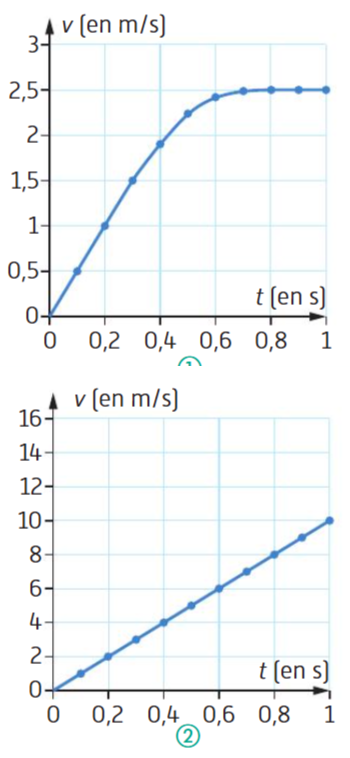
\includegraphics[width=\textwidth]{images/doc3.png}
\end{minipage}%

  \awesomebox[black]{1pt}{\faCogs}{black}{Chute d'une plume et d'une boule de bowling dans une chambre à vide \raisebox{-3.2
ex}{
\includegraphics[scale=0.25]{images/doc4.png}}}

\vfill 
\hrule

\begin{center}
 \LARGE{Activité 3 - Quelle est l'accélération d'un monte charge ? }
\end{center}

\normalsize

\hrule\

\vspace{3mm}
\noindent%
\begin{minipage}{.50\textwidth}%

Un grue est doté d'un variateur de vitesse électronique pour que la montée des charges s'effectue sans à-coup. 
 \ding{202} Déduisez du diagramme des vitesse la nature des trois phases de la montée. 
 \begin{multicols}{3}
  \cadreblanc{10}
  \cadreblanc{10}
  \cadreblanc{10}
  \end{multicols}



\end{minipage}%
\hfill
\begin{minipage}{.45\textwidth}%
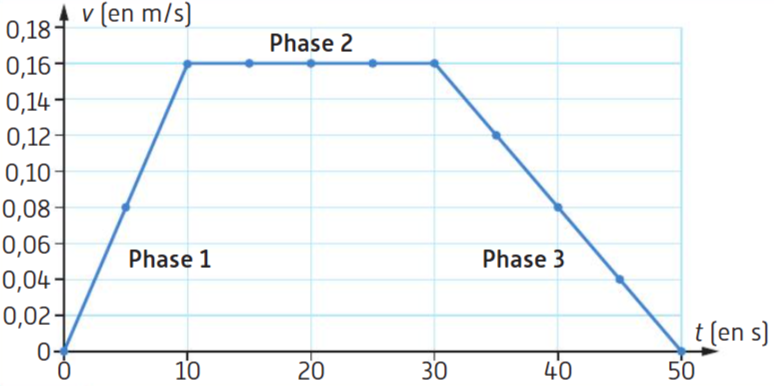
\includegraphics[width=\textwidth]{images/doc5.png}
\end{minipage}%

\vspace{3mm}

\ding{203} Calculez l'accélération de la grue pendant chaque phase, sachant que l'accélération $a$ entre deux points A et B d'une phase est définie par $$a=\dfrac{v_B-v_A}{t_B-t_A}$$
 \begin{multicols}{3}
  \cadreblanc{10}
  \cadreblanc{10}
  \cadreblanc{10}
  \end{multicols}

\ding{204} Expliquez en quoi correspond une accélération négative. 
\cadreblanc{10}




\end{document}